\subsection{Principle of LIGO}

When the gravitational wave reach us, without a doubt, they are only very weak perturbations on our local flat space. Be that as it may, they will provide information about the strong-field regions where they began. it will additionally permit us to decide the wave properties of the gravitational radiation—for ex-sufficient, their spread speed and polarization states \cite{barish1999ligo}. The essential construction of LIGO's interferometers differs a little from the interferometer that Michelson planned more than 125 years prior, however for certain additional highlights. The visible pattern occurring where the coherent waves intersect is simply an "interference" pattern.\cite{collaboration2015advanced}

\subsubsection{Interference Pattern}

In  nature,  the  peaks  and  troughs  of  one  wave cannot absolutely  meet  the  peaks or  troughs  of  another  wave. Regardless  of  how in-sync they are once they merge, the peak of the wave coming out from the interference always equals the sum of the heights of the merging waves on every point wherever they are physically interacting. What  dictates how  well-aligned  the  beams are once  they  merge  is  the path length  they travel before merging. So the core principle of LIGO is interference of light. When the path difference between two light wave is equal to integral multiple of wavelength, then constructive interference occurs where the resultant light will have maximum brightness. And if the path difference is equal to half-integral multiple of wavelength, then destructive interference occurs and resultant light will have minimum brightness. \\

If the beams travel precisely the same distance, their light waves will be absolutely aligned such that they lead to total destructive interference (LIGO is designed to get total destructive interference if no gravitational waves are detected).  But if the lasers don’t travel identical distances, their light waves are not any longer in synchronize as they merge, which implies no light, a bit light, or a light as bright because the original laser beam reaches the photodetector.  And if the arms are changing length over time, a flicker appears as the beams suffer a variety of interference. This time difference is manifested within the interference pattern once the two laser beams superimpose on the path to the photodetector, which can quantify stage movements to ten-billionths of an interference fringe.\cite{barish1999ligo}\\

\begin{figure}[htpb]
    \centering
    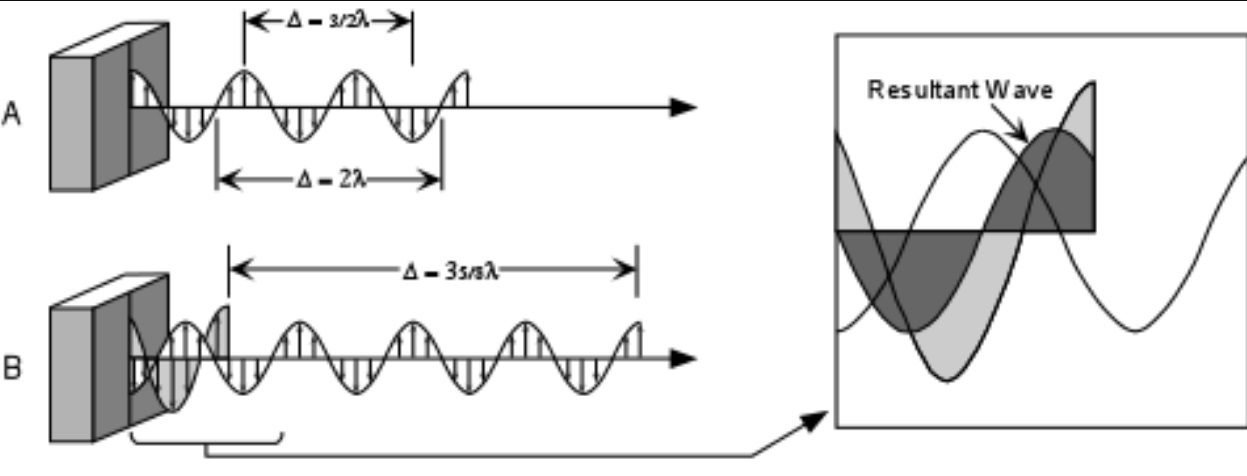
\includegraphics[scale=0.585]{gw-physics-and-ligo/images.tex/interference.jpg}
    \caption{Interference. Source :- \href{https://www.tulane.edu/~sanelson/eens211/interference_of_light.htm}{Interference Phenomena by Prof. Stephen A. Nelson}}
\end{figure}

\subsubsection{How are Gravitational Waves Detected?}

The gravitational waves result in the space to stretch in a direction, at the same time,  compress in a direction perpendicular to it. In LIGO, this results in one arm getting longer whereas the opposite gets shorter, then the other way around, back and forth as long because the wave is passing.  The technical term for this motion is “Differential Arm” motion, or differential displacement, since the arms are at the same time are differing in lengths in opposing ways in which, or deferentially. So because the lengths of the arms differ, thus too will the total path traveled by every laser beam.

\begin{figure}[h]
    \centering
    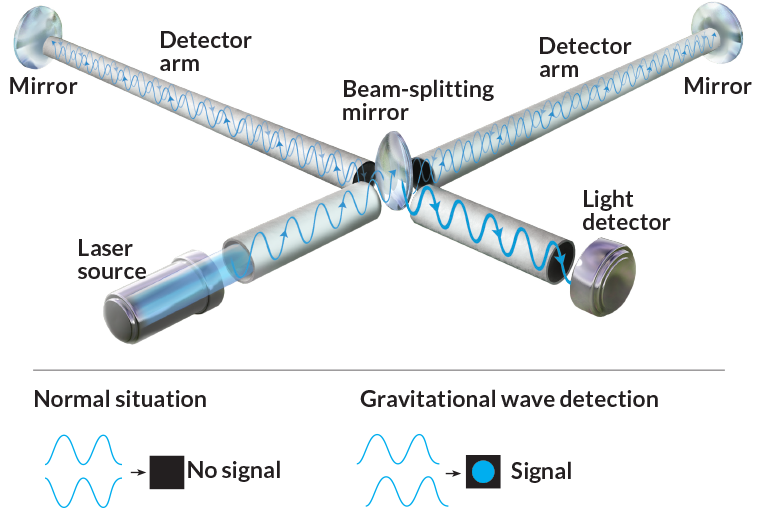
\includegraphics[scale=0.52]{gw-physics-and-ligo/images.tex/Interferometer.jpg}
    \caption{Michelson interferometer.\; Source :- \href{https://www.sciencenews.org/article/trio-wins-physics-nobel-prize-gravitational-wave-detection}{Sciencenews.org}}
\end{figure}

So because the lengths of the arms change, so too does the space traveled by each beam . A beam travelling in the shorter arm will return to the beam splitter before the beam which is ravelling in the extended arm, then things switches because the arms oscillate between being longer and shorter. Arriving at different times, then the LASER does not meet nicely when recombined at the beam splitter. Instead, they shift in and out of alignment or "phase" as they merge. Unlike optical or radio telescopes, LIGO doesn't see electromagnetic waves. It doesn't need to because gravitational waves aren't a part of the spectrum. In fact, electromagnetic wave is so unimportant to LIGO that its detector components are completely isolated and sheltered from the surface world.

\pagebreak
